\documentclass[aspectratio=169]{beamer}

\title{Securing the Django Admin}
\author{David Fischer (djfische@gmail.com)}
\date{February 26, 2020}

%% Beamer Themes
\usetheme{Berlin}
\usecolortheme{dove}
\usefonttheme{serif}

%% Remove beamer controls
\beamertemplatenavigationsymbolsempty

%% Packages
% Pygments must be accessible to use minted and --shell-escape
%  must be used with pdflatex
\usepackage{minted}
\usepackage{hyperref}
\usepackage{multicol}
\usepackage[font=scriptsize,labelformat=empty]{caption}


\setbeamertemplate{footline}{
  \hspace*{.2cm}
  \scriptsize{
    \insertshorttitle
    \hspace*{50pt}
    \hfill
    \insertframenumber/\inserttotalframenumber
    \hspace*{.2cm}
  }
  \vspace{9pt}
}




\begin{document}

\maketitle


\begin{frame}
  \begin{figure}[p]
    \centering
    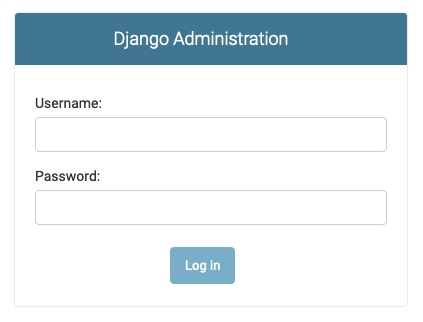
\includegraphics[width=0.5\paperwidth]{images/securing-django-admin-login.png}
  \end{figure}
\end{frame}


\begin{frame}
\frametitle{Django deployment musts}
  \begin{itemize}
    \item Keep the SECRET\_KEY a secret
    \item Never run DEBUG = True on the public internet
    \item Run ``./manage.py check —deploy'' in production
    \item Check out the \href{https://docs.djangoproject.com/en/2.2/howto/deployment/checklist/}{Django deployment checklist}
    \item Read the \href{https://docs.djangoproject.com/en/2.2/topics/security/}{Django security docs}
  \end{itemize}
\end{frame}


\begin{frame}[fragile]
\frametitle{Django settings for production and development}

\begin{multicols}{2}

{\tiny
\begin{minted}{python}
## settings/base.py

INSTALLED_APPS = [
    # ...
]

MIDDLEWARE = [
    # ...
]

LANGUAGE_CODE = "en-us"
TIME_ZONE = "UTC"
USE_I18N = True
USE_L10N = True
USE_TZ = True
\end{minted}
}

\columnbreak

{\tiny
\begin{minted}{python}
## settings/dev.py

from .base import *

# Enable django-debug-toolbar
MIDDLEWARE += ["debug_toolbar.middleware.DebugToolbarMiddleware"]
INSTALLED_APPS += ["debug_toolbar"]


## settings/prod.py

from .base import *
import environ

env = environ.Env()

SECRET_KEY = env("SECRET_KEY")
ALLOWED_HOSTS = env.list("ALLOWED_HOSTS")
DEBUG = False
TEMPLATE_DEBUG = DEBUG

\end{minted}
}

\end{multicols}

\end{frame}





\begin{frame}
\frametitle{Only serve the admin over HTTPS}
  \begin{figure}[p]
    \centering
    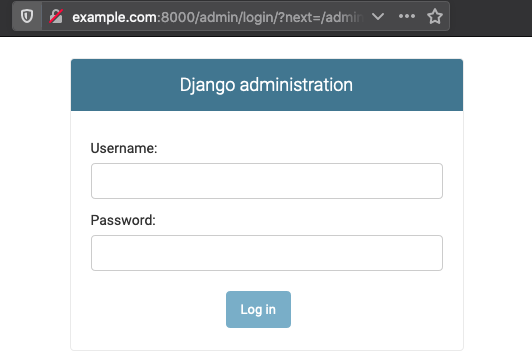
\includegraphics[width=0.6\paperwidth]{images/securing-admin-https.png}
  \end{figure}
\end{frame}


\begin{frame}[fragile]
\frametitle{HTTPS settings}

{\tiny
\begin{minted}{python}
## settings/prod.py

# Only send cookies over HTTPS
SESSION_COOKIE_SECURE = True
CSRF_COOKIE_SECURE = True

# Always redirect HTTP -> HTTPS
SECURE_SSL_REDIRECT = True

# There are more Django security settings
# Did you run ./manage.py check --deploy ?
\end{minted}
}

\end{frame}


\begin{frame}
  \begin{figure}[p]
    \centering
    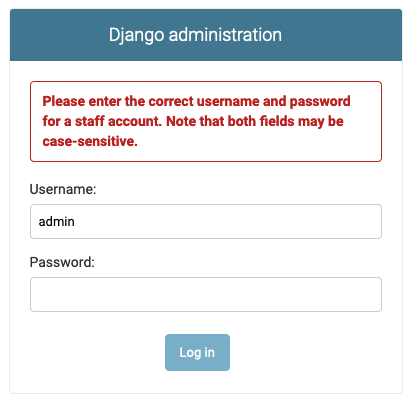
\includegraphics[width=0.4\paperwidth]{images/securing-admin-brute-force.png}
  \end{figure}
\end{frame}


\begin{frame}[fragile]
\frametitle{Selectively enabling the Django Admin}

{\tiny
\begin{minted}{python}
## urls.py

if settings.ADMIN_ENABLED:
    urlpatterns += [
        path(f"{settings.ADMIN_URL}/", admin.site.urls),
    ]


## settings/base.py

ADMIN_ENABLED = env.bool("ADMIN_ENABLED", default=True)
ADMIN_URL = env("ADMIN_URL", default="admin")
\end{minted}
}

\end{frame}



% Peter's talk goes into more including scaling and deploying
% but the section on securing is good
\begin{frame}
\frametitle{Resources}
  \begin{itemize}
    \item {\small \href{https://2019.djangocon.us/talks/prepping-your-project-for-production/}{Prepping Your Project for Production (Peter Baumgartner - Djangocon US 2019)}}
    \item {\small \href{https://developer.mozilla.org/en-US/docs/Learn/Server-side/Django/Deployment}{Mozilla's Django deployment tutorial}}
    \item {\small \href{https://docs.djangoproject.com/en/2.2/howto/deployment/checklist/}{Django deployment checklist}}
    \item {\small \href{https://docs.djangoproject.com/en/2.2/topics/security/}{Django security docs}}
    \item {\small \href{https://observatory.mozilla.org/}{Mozilla Observatory}}
  \end{itemize}
\end{frame}


\begin{frame}
\frametitle{Interested in more Django Admin talks?}
  Past Talks
  \begin{itemize}
    \item {\small \href{https://github.com/davidfischer/talk-customizing-django-admin}{Customizing the Django Admin}}
    \item {\small \href{https://github.com/davidfischer/talk-optimizing-django-admin}{Optimizing the Django Admin}}
  \end{itemize}

  \vfill

  Future Talks
  \begin{itemize}
    \item {\small Django Admin Add-Ons \& Extensions}
  \end{itemize}
\end{frame}


\begin{frame}
\frametitle{}
  {\huge Questions or comments?}
\end{frame}


\end{document}
